\documentclass[tikz, border=3mm]{standalone}
\usepackage{tikz}
\usetikzlibrary{arrows.meta, positioning}

\begin{document}
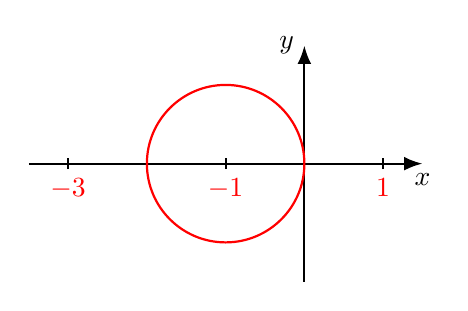
\begin{tikzpicture}[
    >=Latex, % Set default arrow tip style
    axis/.style={->, thick}, % Style for axes
    pathstyle/.style={red, thick}, % Style for the circle path
    labelstyle/.style={red}, % Style for labels
    tick/.style={thick} % Style for tick marks
]

    % Define circle parameters based on image
    % Passes through 0 and -2, so center is -1, radius is 1
    \coordinate (Center) at (-1, 0);
    \def\radius{1}

    % Axes (adjust limits to include ticks)
    \draw[axis] (-3.5, 0) -- (1.5, 0) node[below] {$x$};
    \draw[axis] (0, -1.5) -- (0, 1.5) node[left] {$y$};

    % Draw the red circle
    \draw[pathstyle] (Center) circle (\radius);

    % Ticks and Labels on x-axis
    \foreach \x in {-3, -1, 1} {
        \draw[tick] (\x, -2pt) -- (\x, 2pt);
        \node[labelstyle, below=2pt] at (\x, 0) {$\x$};
    }

\end{tikzpicture}
\end{document}